%% packages
\documentclass{article}
\usepackage[a4paper, left=2.0cm, right=2.0cm, top=3.5cm]{geometry}
\usepackage[ngerman]{babel}
\usepackage{graphicx}
\usepackage{multicol}
\usepackage{amssymb}
\usepackage{titlesec}
\usepackage{wrapfig}
\usepackage{blindtext}
\usepackage{lipsum}
\usepackage{caption}
\usepackage{listings}
\usepackage{fancyhdr}
\usepackage{nopageno}
\usepackage{authblk}
\usepackage{amsmath} % tons of math stuff
\usepackage{mathtools} % e.g. alignment within matrix
%\usepackage{bm} % provides shorthand for bold in math mode
\usepackage{dsfont} % \mathds makes double stroke digits
\usepackage{esdiff} % provides \diff
%\usepackage[ISO]{diffcoeff}
\usepackage{xcolor}
\usepackage{csquotes} % e.g. provides \enquote
\usepackage[separate-uncertainty=true]{siunitx} % units
\usepackage{xcolor} % colored text
\usepackage{csvsimple}
\usepackage{subcaption}
\usepackage{physics}
\usepackage{hyperref}
\usepackage{nameref}
\hypersetup{colorlinks=true, linkcolor=black, pdfhighlight={/N}}
\usepackage{tcolorbox}
\usepackage{amsthm}
\usepackage{float}
\usepackage{enumitem}
\usepackage{booktabs}

% \sisetup{
%   scientific-notation = auto,  % Automatically use scientific notation for large/small numbers
%   output-exponent-marker = \text{e}  % (optional) for formatting the exponent symbol
% }

%\fancyhf[]{}

%% custom stuff
% own units
\DeclareSIUnit \VSS {\ensuremath{V_\mathrm{SS}}}
\DeclareSIUnit \VS {\ensuremath{V_\mathrm{S}}}
\DeclareSIUnit \Veff {\ensuremath{V_\mathrm{eff}}}
\DeclareSIUnit \Vpp {\ensuremath{V_\mathrm{pp}}}
\DeclareSIUnit \Vp {\ensuremath{V_\mathrm{p}}}
\DeclareSIUnit \VRMS {\ensuremath{V_\mathrm{RMS}}}
\DeclareSIUnit \ASS {\ensuremath{A_\mathrm{SS}}}
\DeclareSIUnit \AS {\ensuremath{A_\mathrm{S}}}
\DeclareSIUnit \Aeff {\ensuremath{A_\mathrm{eff}}}
\DeclareSIUnit \App {\ensuremath{A_\mathrm{pp}}}
\DeclareSIUnit \Ap {\ensuremath{A_\mathrm{p}}}
\DeclareSIUnit \ARMS {\ensuremath{A_\mathrm{RMS}}}

% change subsection numbering to capital letters
\newcommand{\subsectionAlph}{ \renewcommand{\thesubsection}{\arabic{section}.\Alph{subsection}} }
% change subsection numbering to lowercase letters
\newcommand{\subsectionalph}{ \renewcommand{\thesubsection}{\arabic{section}.\alph{subsection}} }
% change subsubsection numbering to lowercase letters
\newcommand{\subsubsectionalph}{ \renewcommand{\thesubsubsection}{\arabic{section}.\arabic{subsection}.\alph{subsubsection}} }
% own fig. that works with multicols
\newenvironment{Figure}
  {\par\medskip\noindent\minipage{\linewidth}}
  {\endminipage\par\medskip}
\newcommand*{\inputPath}{./plot} % prepend this command to the argument of all input commands
\graphicspath{ {./images/}{./figure/}{../plot/}{../../plot/}{../../latex/assets/}{./assets/} }
% own enviroment for definitions
\newenvironment{definition}[1]
{\begin{quote} \noindent \textbf{\textit{#1\ifx&#1& \else : \fi}} \itshape}
{\end{quote}}



% own commands
% \newcommand{\rarr}{$\to\,$} %A$\,\to\,$B
\newcommand{\defc}{black}
\newcommand{\colorT}[2][blue]{\color{#1}{#2}\color{\defc}}
\newcommand{\redq}{\color{red}(?)\color{\defc}}
\newcommand{\question}[1]{\colorT[purple]{\textbf{(#1)}}}
\newcommand{\todo}[1]{\colorT[red]{\textbf{(#1)}}}
\newcommand{\mr}{\mathrm}


%% preparation


%dachte wir können hier durchführung und gleich Auswertung der einzelnen Versuchsaufgaben schreiben und im Fazit ein gesamtfazit

%\displaystyle \lim_{x \to \infty}

\begin{document}
\begin{titlepage}
    \title{Elektronikpraktikum \\ Versuch 0: Einführung und Vorversuch}
    \author[1]{Carlos Pascua\thanks{s87cpasc@uni-bonn.de}}
    \author[1]{Anna Maróti\thanks{s32amaro@uni-bonn.de}}
    \author[1]{Cornelius Heiming\thanks{s64cheim@uni-bonn.de}}
    \affil[1]{Uni Bonn}
    %\date{\today}
\end{titlepage}
	\pagenumbering{gobble}
\maketitle
\tableofcontents
\newpage
\pagenumbering{arabic}

\pagestyle{fancy}
\fancyhead[R]{\thepage}
\fancyhead[L]{\leftmark}

\section{Theorie}

\subsection*{Einführung}

In diesem Versuch wird die Ausbreitung von Signalen in verschiedenen Kabeln, wie beispielsweise in Koaxialkabeln, untersucht. Des Weiteren werden Wechselspannungssignale bei verschiedenen Widerständen und unterschiedlichen Leitungsenden analysiert, um ihr Verhalten zu verstehen
??
%Jegliche Schaltkreise, sowie das Diagramm \ref{Dämpfung Kabelsorten Diagramm} entstammen aus \cite{skript:ElektronikPraktikum}.
% das hatten noah und ich das letzte mal geschrieben um das skript zu zitieren. aber hier haben wir eine andere Zitierform


\subsection*{Koaxialleiter}

Ein Koaxialleiter setzt sich aus einem inneren und einem äußeren zylindrischen Leiter zusammen. Sie sind konzentrisch angeordnet und werden von einem Dielektrikum voneinander getrennt. Das Dielektrikum isoliert die Leiter voneinander, welches die Signalübertragung unterstützt, da es die elektrische Feldstärke zwischen den Leitern minimiert wird. 
Die Kapazität und Induktivität von einem Koaxialleiter entspricht:

    \begin{equation}
        C= \epsilon_r \epsilon_0 l \frac{2\pi}{\ln{\frac{R_a}{R_i}}}
    \end{equation}
    
    \begin{equation}
        L= \mu_r \mu_0  \frac{\ln{R_a/R_i}}{2\pi}
    \end{equation}
    
wobei $l$ Länge des Kabels, $R_{a/i}$ Radien der Leitern,$\epsilon_0 = 8,85\cdot10^{-12} \frac{As}{Vm}$ die elektrische Feldkonstante und $\mu_0 = 4\pi\cdot 10^{-7} \frac{Vs}{Am}$ die magnetischen Feldkonstante ist.


Den Kabel kann man auch als mehreren zusammenhängenden LC-Gliedern approximieren. Die Länge L bestimmt dann nicht nur  $C$ und $L$, sondern hat auch einen proportionalen Einfluss auf die Impedanz und Admittanz des Kabels. Eine Weitere wichtige Größe ist der Verlustleitwert (Ableitung) $G$. Dieser ist der ohmsche Leitwert zwischen dem Hin- und Rückleiter. \\
Des Weiteren gibt wird der Kabel noch über seine Übertragungsfähigkeit bestimmt, welches durch den Wellenwiderstand Z, der Verzögerungszeit und der Dämpfung definiert ist. Für den Wellenwiderstand gilt mit der Induktivität $L^{\prime}$ und Kapazität $C^{\prime}$ pro Längeneinheit:
\[ Z = \sqrt{\frac{L^{\prime}}{C^{\prime}}}= \sqrt{\frac{\mu_r \mu_0}{\epsilon_r \epsilon_0}}\cdot \frac{\ln{R_a/R_i}}{2\pi}\]
Die Verzögerungszeit setzt sich aus der Zeitdifferenz der einlaufenden und reflektierten Welle zusammen. 
Und die Dämpfung ist gegeben mit der Dämpfungskonstante $ \alpha$ durch:
\begin{equation*}
    \Upsilon = \alpha + i \beta
\end{equation*}

\subsection*{Wellenausbreitung und Leitungsabschluss}
Anhand des Superpositionprinzips können Strom und Spannung durch eine Überlagerung einer hin- und \\ rücklaufenden Welle beschrieben werden.
\begin{equation*}
   U(x,t) = U_h(x,t) + U_r(x,t)= (U_{h0} e ^{-\Upsilon x} + U_{r0} e ^{-\Upsilon x}) e^{i \omega t} 
\end{equation*}
und 
\begin{equation*}
    I(x,t) = (U_{h0} e^{-\Upsilon x} + U_{r0} e^{-\Upsilon x}) \cdot \sqrt{\frac{G^{\prime}+ i \omega C^{\prime}}{R^{\prime}+ i \omega L^{\prime}}}e^{i \omega t}= I_h(x,t) + I_r(x,t)
\end{equation*}
Aus diesem Grund spielt der Leitungsabschluss und dessen Reflektionsgrad eine signifikante Rolle in der Elektrotechnik.

\subsection*{Angepasster Anschluss}
$R_A = Z$\\
Der Abschlusswiderstand $R_A$ entspricht dem Wellenwiderstand $Z$ des Kabels. Hierdurch überträgt sich die gesamte Energie des Kabels an den Verbraucher und die Welle wird nicht reflektiert, da der Verbraucher wie eine Weiterführung des Kabels entspricht und die Welle weiter den Kabel durchdringt.


\subsection*{Offene Leitung}
$R_A = \infty$\\
Es wird kein Strom an den Verbraucher übertragen, da der Abschlusswiderstand Unendlich entspricht. Hierdurch wird die gesamte Energie der Welle in gleicher Phase zurückreflektiert. Die rücklaufende Welle ist genau so groß wie die hinlaufende Welle.



\subsection*{Kurzschluss }
$R_A= 0 \Omega$\\
Bei einem Kurzschluss entspricht der der Abschlusswiderstand $ 0 \Omega$. Hierdurch wird die rücklaufende Welle phasenverschoben reflektiert. Sie entspricht der Inversen der hinlaufenden Welle, weshalb die beiden Wellen sich destruktiv überlagern und die Spannung 0 V ergibt.

\section{Voraufgaben}

\subsection*{Aufgabe A}
Um möglichst große Verzögerungszeiten zu bekommen, muss die Phasengeschwindigkeit verkleinert werden und die Leitungslänge l vergrößert werden. Außerdem haben weitere Parameter einen Einfluss auf die Vergrößerungszeit

\begin{equation}
    v_{ph}= \frac{1}{\sqrt{L^{\prime}C^{\prime}}}= \frac{1}{\epsilon_0\mu_0}\cdot \frac{1}{\epsilon_r\mu_r} =c_0 \cdot \frac{1}{\epsilon_r\mu_r}
\end{equation}

Also ist $t \propto L^{\prime}\propto C^{\prime}$. Außerdem kann man ableiten, dass man für eine große Verzögerungszeit das Kabel ein hohes Dielektrikum haben sollte, da dieses die Dielektrizität und Permeabilität erhöht wozu t auch proportional ist. 


\subsection*{Aufgabe B}
Der Wellenwiderstand kann durch folgende Formel beschrieben werden 
\begin{equation}
    Z = \sqrt{\frac{L^{\prime}}{C^{\prime}}} = \frac{\mu_0 \mu_r}{\epsilon_0\epsilon_r}\cdot \frac{\ln{\frac{R_a}{R_i}}}{2\pi}
\end{equation}

Also hat die Veränderung der Verzögerungszeit durch die Parameter aus Aufgabe A, eine Auswirkung auf den Wellenwiderstand.Wenn die Induktivität oder Permeattivität erhöht wird, dann erhöht sich der Wellenwiderstand. Falls die Kapazität oder die Dielektrizität erhöht werden, verkleinert sich der Wellenwiderstand. Die Leitungslänge l hat keinen Einfluss auf den Widerstand.


\subsection*{Aufgabe C}
Der Eingangswiderstand ist unabhängig vom Kabel, falls das Kabel abgeschlossen ist und $R_A = Z$, da dann $R_A = Z= R_{in}$


\subsection*{Aufgabe D}

Folgende Eigenschaften sind einem Leiter im Idealfall gegeben: $\frac{\mathrm{R_A}}{\mathrm{R_1}} = 2,3$, $\epsilon_0 = 1,5$, $\mu_0 = 1,5$. 
\\
Für die Phasengeschwindigkeit $v_{ph}$ gilt: 
\begin{equation*}
    v_{ph} = \frac{1}{\sqrt{L'\cdot C'}} = \frac{1}{\sqrt{\epsilon_r \epsilon_0 \mu_r \mu_0}} = c_o \cdot \frac{1}{\sqrt{\epsilon_r \mu_r}} = 2 \cdot 10^8  \frac{m}{s} 
\end{equation*}
Für den Wellenwiderstand gilt:
\begin{equation}
    Z = \sqrt{{\frac{L'}{C'}}} = Z_{frei} \cdot \frac{\ln(\frac{R_A}{R_1})}{2\pi} \approx 49,98\Omega
\end{equation}

Somit ergibt sich für die Verzögerungszeit pro Meter: $t_v = 5 \cdot 10^{-9}$

\section{Versuchsaufbau, -durchführung, Messwerte und Auswertung}
		Zunächst werden die Seriennummern der verwendeten Laborgeräte notiert.
		
		
% === Aufgabe 1 ===
		\subsection{Versuchsaufgabe 1: Differenzierglied}


			\begin{figure}[H]
				\centering
				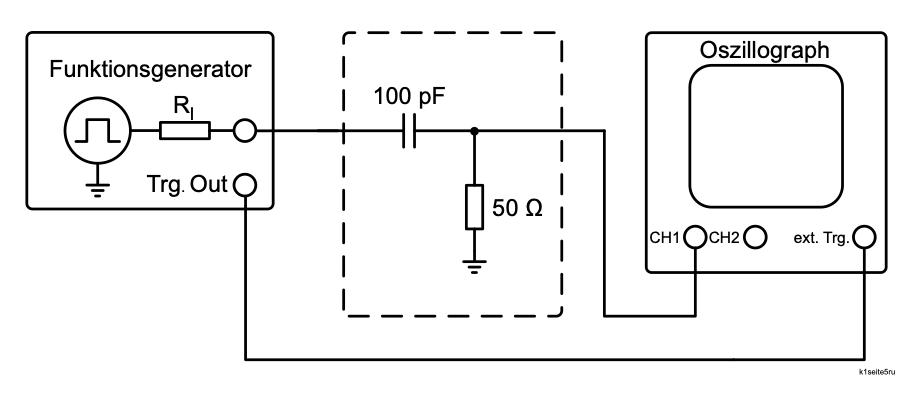
\includegraphics[width=0.8\textwidth]{figs/Aufbau_1_1_Differenzierglied.png}
				\caption{Schaltplan eines Differenzierglieds~\cite{anleitung}}
				\label{fig:aufbau_1_1_differenzierglied}
			\end{figure}
			Ein RC-Glied wird (ohne $\SI{2.2}{\kilo\ohm}$ Abschluss) zwischen einen Funktionsgenerator und einen Oszillographen geschaltet. Der Funktionsgenerator wird auf eine Frequenz von $\SI{200}{\kilo\hertz}$ eingestellt. Dann wird das Oszillogramm gezeichnet und dasselbe mit dem $\SI{2.2}{\kilo\ohm}$ Abschlusswiderstand wiederholt.
			
			
			\begin{figure}[H]
				\centering
				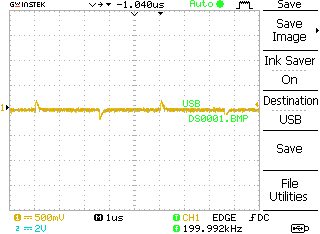
\includegraphics[width=0.8\textwidth]{MesswerteVersuch1/DS0001.png}
				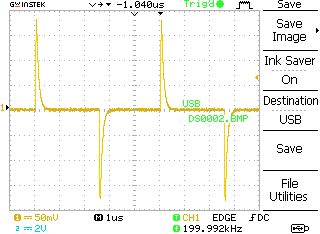
\includegraphics[width=0.8\textwidth]{MesswerteVersuch1/DS0002.png}
				\caption{Differenzierglied mit Abschlusswiderstand (unten vergrößerte Ordinate)}
				\label{fig:DS0001,2}
			\end{figure}
			\begin{figure}[H]
				\centering
				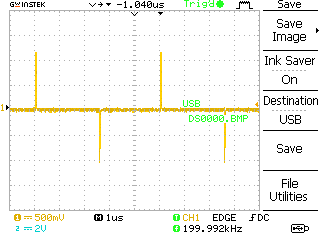
\includegraphics[width=0.8\textwidth]{MesswerteVersuch1/DS0000.png}
				\caption{Differenzierglied ohne Abschlusswiderstand}
				\label{fig:DS0000}
			\end{figure}
			
				Wie in \ref{fig:DS0000} zu erkennen ist, wird das Rechtecksignal des Funktionsgenerators durch das Differenzierglied in ein Impulsignal umgewandelt. Die Spikes sind hierbei gut zu erkennen. Dies ist im Fall mit dem Abschlusswiderstand anders, dort "schluckt" das Differenzierglied die Impulse (vgl. \ref{fig:DS0001,2} oben), diese sind nur noch wesentlich schwächer zu sehen (vgl. \ref{fig:DS0001,2} unten). Dies ist darauf zurückzuführen, dass der Abschlusswiderstand den Stromfluss behindert und somit die Impulse nicht mehr so stark ausgeprägt sind. Der Abschlusswiderstand hat also eine dämpfende Wirkung auf das Signal.

			%TODO: Messwerte & Auswertung
	
\clearpage
% === Aufgabe 2 ===

\subsection{Versuchsaufgabe 2: Impulse auf Kabeln} 

			
			\begin{figure}[H]
				\centering
				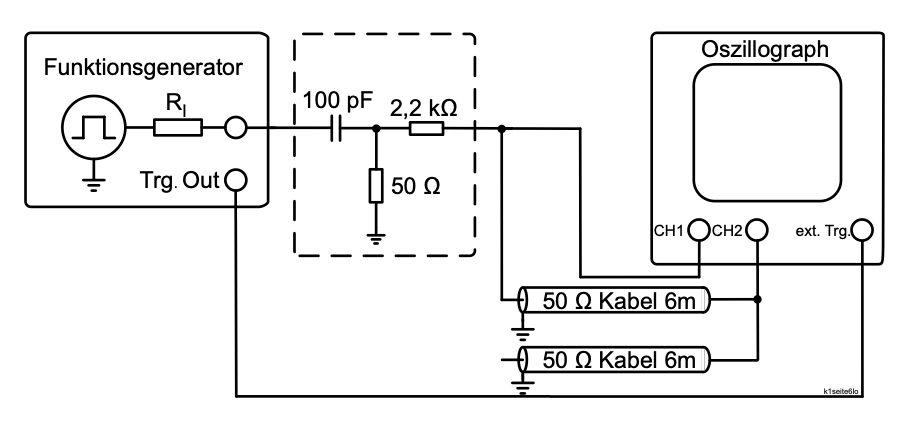
\includegraphics[width=0.8\textwidth]{figs/Aufbau_1_2_Impulse_auf_Kabeln.png}
				\caption{Schaltplan für ein Kabel mit zwei offenen Enden~\cite{anleitung}}
				\label{fig:aufbau_1_1_impulseAufKabeln}
			\end{figure}
			Jetzt sollen die Impulse auf einem an beiden Enden offenen Kabel untersucht werden. Dazu wird ein Funktionsgenerator, welcher im Rechteckmodus mit $\SI{100}{\kilo\hertz}$ betrieben wird, vor ein RC-Glied mit Abschluss, welches als Impulsgeber dient, geschaltet. Diese Impulse werden einerseits im CH1 des Oszillographen angezeigt, andererseits durch zwei hintereinandergeschaltete Kabel mit jeweils $\SI{50}{\ohm}$ Wellenwiderstand geschickt. Zwischen den beiden Kabeln wird der Oszillograph im CH2 geschaltet. Der Funktionsgenerator dient als externer Trigger für den Oszillographen, die beiden Kanäle werden mit derselben Empfindlichkeit betrieben.
			
			Auf der größeren Zeitachse (vgl. \ref{fig:DS0004}) kann man die Impulse des Funktionsgenerators wiedererkennen. Hier klingen diese nicht instantan durch die Darstellung im Oszillographen ab, sondern wandern durch die beiden Kabel, sodass nur ein Teil der Amplitude im Oszillographen ankommt. In der detaillierteren Darstellung (vgl. \ref{fig:DS0005}) kann man nun die einzelnen Durchläufe durch die beiden Kabel erkennen. Besonders gut dabei zu sehen ist, dass der Impuls den Punkt zwischen den beiden Kabeln doppelt so häufig passiert, wie den Punkt am Anfang des Kabels. Das macht also eine tatsächliche Bewegung des Signales über die Länge der Kabel deutlich. Dies kann man auch aus der Verzögerung der beiden Signale relativ zueinander erkennen, die in etwa der Hälfte der Periode vom Mittelpunkt bzw. einem Viertel der Periode vom Anfang des Kabels entspricht. 
			
			\begin{figure}[H]
				\centering
				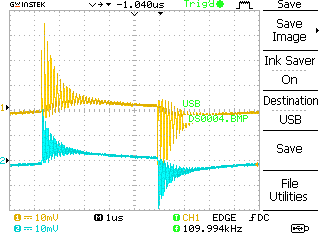
\includegraphics[width=0.8\textwidth]{MesswerteVersuch1/DS0004.png}
				\caption{Impulse auf Kabeln (Übersicht ($\SI{1}{\micro\second\per\centi\meter}$))}
				\label{fig:DS0004}
			\end{figure}
			\begin{figure}[H]
				\centering
				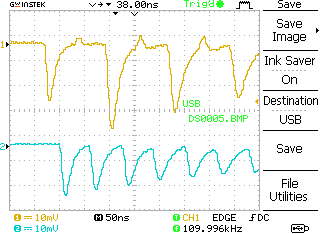
\includegraphics[width=0.8\textwidth]{MesswerteVersuch1/DS0005.png}
				\caption{Impulse auf Kabeln (Detailansicht ($\SI{0.05}{\micro\second\per\centi\meter}$))}
				\label{fig:DS0005}
			\end{figure}
		
\clearpage
% === Aufgabe 3 ===

\subsection{Versuchsaufgabe 3: Leitungsabschluss, Verzögerungszeit}
			
			\begin{figure}[H]
				\centering
				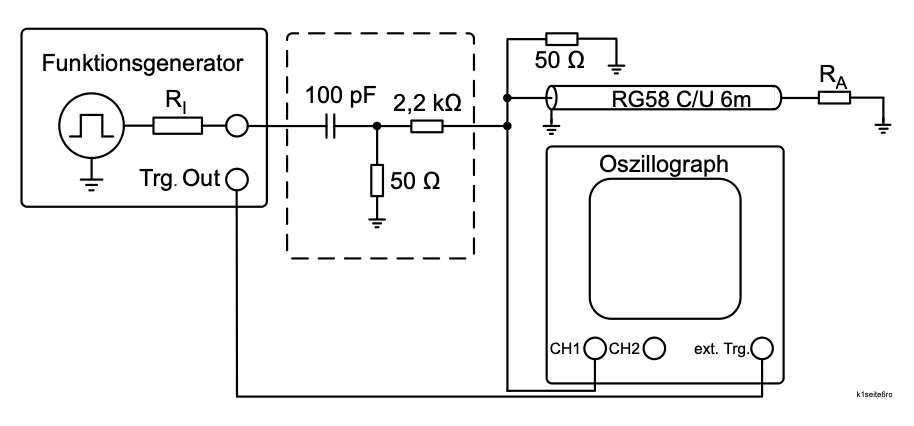
\includegraphics[width=0.8\textwidth]{figs/Aufbau_1_3_Leitungsabschluss.png}
				\caption{Schaltplan für ein Kabel mit einem offenen und einem geschlossenen Ende~\cite{anleitung}}
				\label{fig:aufbau_1_3_leitungsabschluss}
			\end{figure}
			Nun wird die Auswirkung unterschiedlicher Leitungsabschlüsse auf die Impulse untersucht. Dazu wird weiterhin extern getriggert, der Impulsgenerator wird auch an CH1 angeschlossen. Statt der beiden Kabel wird jetzt mittels eines T-Stücks ein Verzögerungskabel mit $\SI{50}{\ohm}$ Wellenwiderstand und $\SI{6}{\meter}$ Länge verwendet, welches am anderen Ende mit einem Widerstand $R_\mathrm{A} = \SI{50}{\ohm}$ abgeschlossen ist. Es für jede der folgenden Anordnungen mit und ohne einem zusätzlichen Widerstand von $\SI{50}{\ohm}$ parallel zum Kabel gemessen:
			\begin{enumerate}[label=\alph*]
				\item Offenes Ende
				\item Offenes Ende im Detail ($\times 10$)
				\item Kurzgeschlossenes Ende
				\item Kurzgeschlossenes Ende \& variierende Frequenzen (Zeitablenktung von $\SI{0.2}{\micro\second\per\centi\meter}$)
			\end{enumerate}

            Durch den Mangel eines Widerstands treten Reflexionen auf, wodurch sich rücklaufende Wellen und hinlaufende Wellen
            überlagern. Dies lässt sich durch die Dämpfung der Kabel erklären. 

				%TODO: Auswertung 3(a)
				\begin{figure}[H]
					\centering
					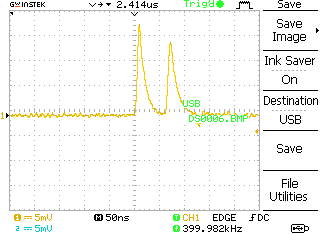
\includegraphics[width=0.5\textwidth]{MesswerteVersuch1/DS0006.png}
					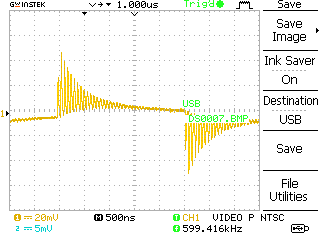
\includegraphics[width=0.5\textwidth]{MesswerteVersuch1/DS0007.png}
					\caption{Leitungsabschluss offenes Ende (oben: mit Anpassunsgwiderstand, unten: ohne Anpassungswiderstand)}
					\label{fig:DS0006,7}
				\end{figure}
 
                Mit der Abbildung \ref*{fig:DS0006,7} lässt sich die abgedämpften Peaks
                zu erkennen. Die Schi

                \clearpage 
				\begin{figure}[H]
					\centering
					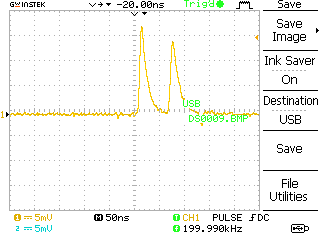
\includegraphics[width=0.8\textwidth]{MesswerteVersuch1/DS0009.png}
					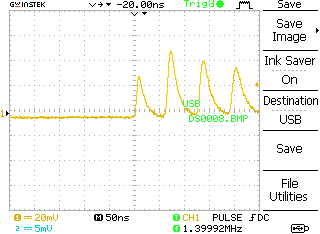
\includegraphics[width=0.8\textwidth]{MesswerteVersuch1/DS0008.png}
					\caption{Leitungsabschluss offenes Ende (oben: mit Anpassunsgwiderstand, unten: ohne Anpassungswiderstand) vergrößert}
					\label{fig:DS0009.8}
				\end{figure}

                

				%TODO: Auswertung 3(b)

				%TODO: Auswertung 3(c)
				\begin{figure}[H]
					\centering
					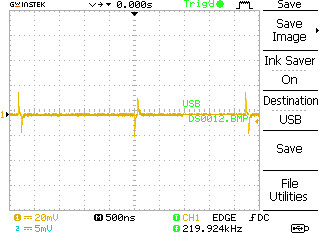
\includegraphics[width=0.8\textwidth]{MesswerteVersuch1/DS0012.png}
					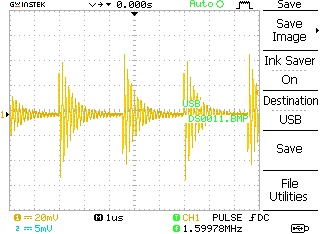
\includegraphics[width=0.8\textwidth]{MesswerteVersuch1/DS0011.png}
					\caption{Leitungsabschluss kurzgeschlossenes Ende (oben: mit Anpassunsgwiderstand, unten: ohne Anpassungswiderstand)}
					\label{fig:DS000}
				\end{figure}
\clearpage
				\begin{figure}[H]
					\centering
					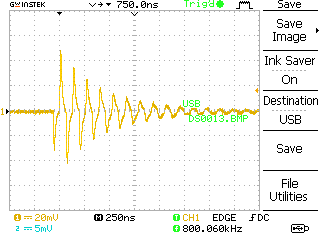
\includegraphics[width=0.8\textwidth]{MesswerteVersuch1/DS0013.png}	

					\caption{Leitungsabschluss kurzgeschlossenes Ende, Frequenz: $\SI{100}{\kilo\hertz}$}
					\label{fig:DS0013}
				\end{figure}
				\begin{figure}[H]
					\centering
					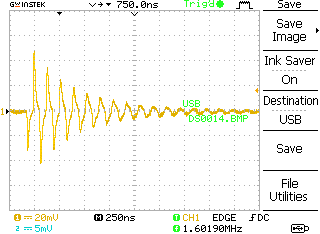
\includegraphics[width=0.8\textwidth]{MesswerteVersuch1/DS0014.png}	

					\caption{Leitungsabschluss kurzgeschlossenes Ende, Frequenz: $\SI{200}{\kilo\hertz}$}
					\label{fig:DS0014}
				\end{figure}
				\begin{figure}[H]
					\centering
					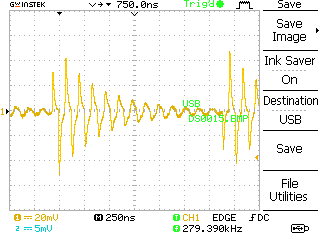
\includegraphics[width=0.8\textwidth]{MesswerteVersuch1/DS0015.png}	

					\caption{Leitungsabschluss kurzgeschlossenes Ende, Frequenz: $\SI{300}{\kilo\hertz}$}
					\label{fig:DS0015}
				\end{figure}
				\begin{figure}[H]
					\centering
					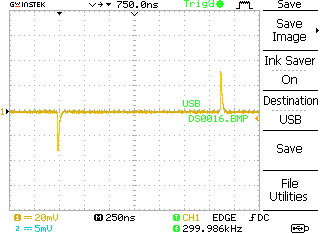
\includegraphics[width=0.8\textwidth]{MesswerteVersuch1/DS0016.png}	

					\caption{Leitungsabschluss mit Wellenwiderstand}
					\label{fig:DS0016}
				\end{figure}
				%TODO: Auswertung 3(d)
\clearpage
% === Aufgabe 4 ===		

\subsection{Versuchsaufgabe 4: Klippkabel, Dämpfung}
			\begin{figure}[H]
				\centering
				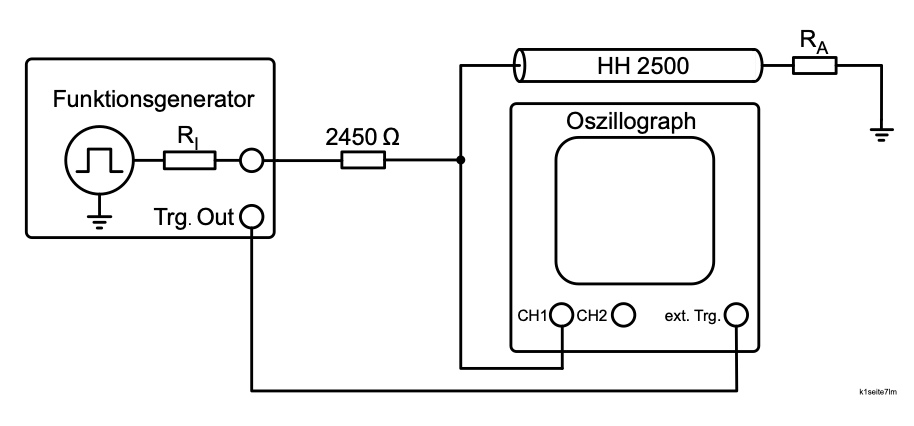
\includegraphics[width=0.8\textwidth]{figs/Aufbau_1_4_Klippkabel.png}
				\caption{Schaltplan für ein Klippkabel~\cite{anleitung}}
				\label{fig:aufbau_1_4_klippkabel}
			\end{figure}
			Zuletzt wird das Verzögerungskabel mit einem kürzeren, sogenannten Klippkabel, mit $\SI{0.7}{\meter}$ Länge ersetzt. Anstatt des Differenzierglieds wird ein Widerstand von $\SI{2450}{\ohm}$ eingebaut, der Widerstand vor dem Kabel wird entfernt. Der Funktionsgenerator wird auf eine Frequenz zwischen $\SI{10}{\kilo\hertz}$ und $\SI{80}{\kilo\hertz}$ eingestellt. Die Schaltverbindungen erfolgen mit $\SI{50}{\ohm}$ Koaxialkabeln. Dann wird unter den folgenden Umständen am Oszillographen gemessen:
			\begin{enumerate}[label=\alph*]
				\item Klippkabel mit $\SI{50}{\ohm}$ Abschluss, d.\ h.\ offen
				\item Klippkabel kurzgeschlossen
				\item Klippkabel kurzgeschlossen mit variierter Frequenz
				\item $\SI{2}{\meter}$ Klippkabel kurzgeschlossen 
			\end{enumerate}

				\begin{figure}[H]
					\centering
					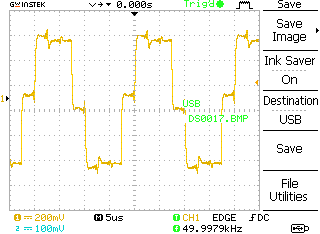
\includegraphics[width=0.8\textwidth]{MesswerteVersuch1/DS0017.png}
					\caption{Klippkabel mit offenem Ende}
					\label{fig:DS0017}
				\end{figure}

				\begin{figure}[H]
					\centering
					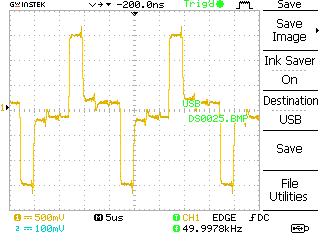
\includegraphics[width=0.8\textwidth]{MesswerteVersuch1/DS0025.png}
					\caption{Klippkabel mit kurzgeschlossenem Ende}
					\label{fig:DS0025}
				\end{figure}

				\begin{figure}[H]
					\centering
					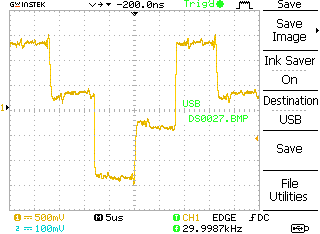
\includegraphics[width=0.8\textwidth]{MesswerteVersuch1/DS0027.png}
					\caption{Klippkabel mit offenem Ende bei $\SI{30}{\kilo\hertz}$}
					\label{fig:DS0030}
				\end{figure}

				\begin{figure}[H]
					\centering
					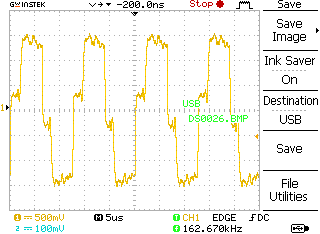
\includegraphics[width=0.8\textwidth]{MesswerteVersuch1/DS0026.png}
					\caption{Klippkabel mit offenem Ende bei $\SI{80}{\kilo\hertz}$}
					\label{fig:DS0030}
				\end{figure}

		
		%TODO Aufbau/Schaltskizze (beschrieben in wenigen Worten)
		%TODO Versuchsdurchführung: Messgrößen, unabh. Parameter, Messmethode, Einheiten, Genauigkeit, wie oft
		%TODO Abgezeichnetes Messprotokoll vorhanden?

		%TODO Auswertung (in Worten & Formeln)
		%TODO Formeln symbolisch und numerisch
		%TODO Runden
		%TODO Grafiken & Diagramme: Überschrift, Messwerte mit Fehlerbalken, (nur) gefittete Kurven, Achsenbeschriftung
		%TODO Fehlerrechnung und -diskussion
		%TODO Jede Tabelle eine Formel
	\section{Fazit}
		%TODO Vollständiger Satz fürs Endergebnis
		%TODO Messergebnisse bewerten und evtl. mit Literaturwerten vergleichen
		%TODO Untersuchung Fehlerquellen (statistisch, systematisch, blödsinnig)




\end{document} 